\documentclass{ximera}
\input{../preamble}
\addPrintStyle{..}
\begin{document}
	\author{Wim Obbels}
	\xmtitle{De norm van een complex getal}{}
	\label{xim:complexe_getallen_norm}


\begin{xmuitweiding}[Over de absolute waarde van een reëel getal]
De absolute waarde $|a|$ van een reëel getal $a$ lijkt op het eerste zicht een tamelijk eenvoudig begrip, want $|a|$ is 'het getal $r$ zonder het teken'.
Op de getallenrechte kan je $|a|$ ook beschouwen als de afstand van $a$ tot de oorsprong, en $|a-b|$ als de afstand tussen $a$ en $b$.
In formules en berekeningen doet de absolute waarde soms vervelend, omdat de absolute waarde $|a+b|$ van een som niet kan geschreven worden als de som van de absolute waarden van de termen, dus als $|a|+|b|$.
\end{xmuitweiding}

%Voor complexe getallen is 'het getal zonder het teken' weinig zinvol, maar de interpretatie als afstand blijkt wel erg nuttig.
%In plaats van over 'absolute waarde' spreekt men bij complexe getallen over de modulus of de norm, en dat zijn eigenlijk andere namen voor 'afstand' bij complexe getallen.

Om het begrip \textit{absolute waarde} $|a|$ van een reëel getal $a\in\R$ te veralgemenen naar complexe getallen begrijp je $|a|$ best als de afstand van het punt $a$ op de reële rechte tot de oorsprong. En bij complexe getallen gebruiken we niet het woord 'absolute waarde', maar wel 'norm' of 'modulus': 


\begin{definition}[Modulus van een complex getal]\label{def:complex_toegevoegde} \nl 
	
De \textbf{modulus} (of \textbf{norm}) van een complex getal $z=a+bi$, genoteerd $|z|$, is het \textit{positief reëel} getal 
%
	\formulevb{|z| \perdef  |a+bi| \perdef \sqrt{a^2+b^2}}{|3+4i| = \sqrt{3^2+4^2} = \sqrt{9+16}=\sqrt{25}=5.}
%

\begin{image}[0.6\textwidth]
	\begin{tikzpicture}[scale=5]%,cap=round,transform canvas={scale=0.5}]
	
	\tikzmath{\hoek = 30;}
	
	\draw[->] (-0.1,0) -- (1.2,0) node[below left] {Re$(z)$};
	\draw[->] (0,-0.1) -- (0,0.7) node[below left] {Im$(z)$};
	
	\draw[color=blue,thick] (0:0)     node[below,black]{$0$} 
	                        --        node[above, rotate=\hoek] {\small $|z|=\sqrt{a^2+b^2}$} 
							(\hoek:1) node [yshift=1pt,above] {$z=a+bi$} ; 
    
	\draw[color=black] (\hoek:1) node[name=P,circle, fill=black, radius=1pt,scale=0.8] {} ;  

    \draw[dashed] ({cos(\hoek)},0) node[below]{$a$} -- (P);
	\draw[dashed] (0,{sin(\hoek)}) node[circle, fill=black, radius=1pt,scale=0.5] {} node[left] {$b$} -- (P);
	\draw[dashed] ({cos(\hoek)},0) node[circle, fill=black, radius=1pt,scale=0.5] {};

	\begin{scope}[xshift=1.5cm]
	
	\draw[color=blue,thick] 
					(0:0)      node[below,black]{$0$}
					--         node[above, rotate=\hoek] {\small $|z|=\sqrt{a^2+b^2}$} 
					(\hoek:1)  node[above,black]{$a+bi$}; 
    
	\draw[color=red] (0,0) -- node[below]{$a$} ({cos(\hoek)},0);  
	\draw[color=red] (\hoek:1) -- node[right]{$b$} ({cos(\hoek)},0);  


	\end{scope}
	
	\end{tikzpicture}
\end{image}

De modulus $|z|$ is meetkundig \textbf{de afstand van $z$ tot de oorsprong} (wegens Pythagoras). 
%en dus ook de \textit{lengte van de vector} $\vec{z}$.
\end{definition}
 
 
\begin{quickquestion*}{}

	Teken alle complexe getallen waarvoor \(|z| = 1\) in het complexe vlak. 
\end{quickquestion*}

% \begin{quickquestion}{}{}    % met een nummer ...
% 	Teken alle complexe getallen waarvoor \(|z| = 1\) in het complexe vlak. 
% \end{quickquestion}

\begin{example}\nl
	\begin{xmmulticols}[4]
		\begin{question} $|i|      = \answer[onlineshowanswerbutton]{1}$        \end{question}
		\begin{question} $|-i|     = \answer[onlineshowanswerbutton]{1}$        \end{question}
		\begin{question} $|-2|     = \answer[onlineshowanswerbutton]{2}$        \end{question}
		\begin{question} $|2i|     = \answer[onlineshowanswerbutton]{2}$        \end{question}
		\begin{question} $|1-1|    = \answer[onlineshowanswerbutton]{0}$        \end{question}
		\begin{question} $|1|+|-1| = \answer[onlineshowanswerbutton]{2}$        \end{question}
		\begin{question} $|3-4i|   = \answer[onlineshowanswerbutton]{5}$        \end{question}
		\begin{question} $|1+i|    = \answer[onlineshowanswerbutton]{\sqrt{2}}$ \end{question}
	\end{xmmulticols}	
\end{example}


\todo{Video verhuizen naar in extra activity 'norm+modulus'}
De meetkundige betekenis van de modulus en complex toegevoegde wordt uitgelegd in onderstaande video:
	
 	\youtube{uSl9oLBjw1U}


De modulus heeft volgende basiseigenschappen, die je allemaal tamelijk eenvoudig kan bewijzen.

\begin{proposition}[Eigenschappen modulus]\label{eig:complexe_modulus}
	Voor complexe getallen $z,z_1,z_2\in \C$ geldt
	%\begin{xmmulticols}
	\begin{enumerate}
		\item $|z|$ is de afstand van $z$ tot de oorsprong.
		\item $|z_1-z_2|$ is de afstand tussen $z_1$ en $z_2$.
		\item $|z|= |-z|$.		
		\item $|z|=0 \iff  z=0 $.
		\item $|z_1\cdot z_2| = |z_1| \cdot |z_2|$.
%		\item $z \cdot \overline{z} = |z|^2$
%		\item $\dfrac{z \cdot \overline{z}}{|z|^2} = 1$ \label{eig:modulus:invers}
		
		%\item $\displaystyle \left| \frac{1}{z}\right|= \frac{1}{|z|}$
		%\item $\left| \displaystyle \frac{z_1}{z_2}\right|=\displaystyle \frac{|z_1|}{|z_2|}$
		%\item \important{|z_1+z_2| \leq |z_1|+|z_2|}
		
	\end{enumerate}
	%
	\todo{Driehoeksongelijkheid terug toevoegen}
	%\end{xmmulticols}
	LET OP: in het algemeen geldt niet $\xcancel{|z_1+z_2| = |z_1|+|z_2|}$ (want bv. $0= |1+(-1)| \neq |1|+|-1| = 2)$
	
\end{proposition}

% Om op één pagina te passen, is het handig de opgave's in de PDF niet te herhalen.
% TODO: misschien toch optioneel de oplossingen in de 'standaard' versie zetten!!!
% \pdfOnly{
% De bewijzen van deze eigenschappen zijn oefeningen. 
% }

\begin{onlineOnly}   % DOES NOT WORK ???
    
\begin{exercise} Bewijs alle uitspraken van Eigenschap~\href{eig:complexe_modulus}.

	\begin{question} 
		$|z|$ is de afstand tussen $z$ en de oorsprong in het complexe vlak.
		\begin{oplossing}
			Het bewijs staat al in Definitie~\ref{def:complex_toegevoegde}.
		\end{oplossing}
	\end{question}
	\begin{question} 
		$|z_1 - z_2|$ is de afstand tussen $z_1$ en $z_2$ in het complexe vlak.
		   
		\begin{oplossing}
			Wegens de parallellogramregel is  $z_1-z_2$  als vector gelijk aan de vector tussen $z_1$ en $z_2$, en dus is $|z_1-z_2|$ ook de afstand tussen $z_1$ en $z_2$.
			\begin{image}[0.4\textwidth]
			    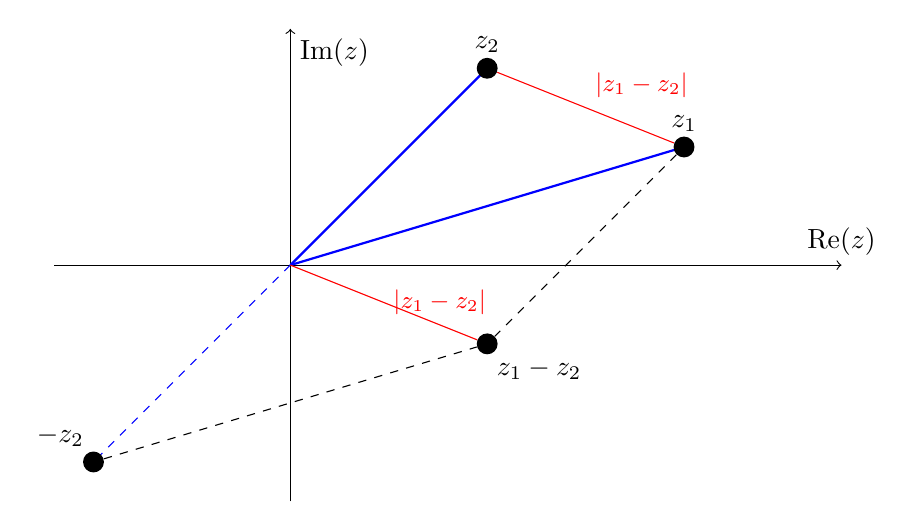
\begin{tikzpicture}[scale=5]%,cap=round,transform canvas={scale=0.5}]
				   
				   \draw[->] (-0.6,0) -- (1.4,0) node[above] {Re$(z)$};
				   \draw[->] (0,-0.6) -- (0,0.6)   node[below right] {Im$(z)$};
				   
				   \draw[color=blue,thick] (0:0)  -- (1,0.3); 
				   \draw[color=blue,thick] (0:0)  -- (0.5,0.5); 
				   \draw[color=blue,dashed] (0:0)  -- (-0.5,-0.5); 			   
				   %
				   \draw[color=black] (1,0.3) node[name=Z1,circle, fill=black, radius=1pt,scale=0.8] {} node [yshift=2pt,above] {$z_1$} ;  
				   \draw[color=black] (0.5,0.5) node[name=Z2,circle, fill=black, radius=1pt,scale=0.8] {} node [yshift=2pt,above] {$z_2$} ;  
				   %
				   \draw[color=black] (-0.5,-0.5) node[name=mZ2,circle, fill=black, radius=1pt,scale=0.8] {} node [yshift=2pt,above left ] {$-z_2$} ;  
				   %
				   \draw[color=black] (0.5,-0.2) node[name=Zv,circle, fill=black, radius=1pt,scale=0.8] {} node [yshift=-2pt,below right] {$z_1-z_2$} ;  
				   %
				   \draw[red] (Z1) -- node[above right] {\small $|z_1-z_2|$} (Z2);
				   \draw[red] (0,0) -- node[right] {\small $|z_1-z_2|$} (Zv);
				   %
				   \draw[dashed] (mZ2) -- (Zv);
				   \draw[dashed] (Z1) -- (Zv);
				   
				\end{tikzpicture}   
			\end{image}
		\end{oplossing}
	\end{question}		   
	
	\begin{question} $|z|= |-z|$.
		\begin{oplossing} Stel $z=a+bi$, bereken beide uitdrukkingen, en stel vast dat ze aan elkaar gelijk zijn.
			\begin{itemize}
				\item $| z| = \sqrt{a^2+b^2}$
				\item $|-z| = \sqrt{(-a)^2+(-b)^2} = \sqrt{a^2+b^2}$ \qed
			\end{itemize}
		\end{oplossing}
	\end{question}
		
	\begin{question} $|z| = 0 \iff z = 0$.
		\begin{oplossing}
			Stel $z=a+bi$, en bewijs de equivalentie door twee implicaties aan te tonen:
			
			1. $\boxed{\Rightarrow}$ Als $|z| = 0$, dan is $a^2+b^2 = 0$,. Omdat kwadraten positief zijn, kan $a^2+b^2=0$  alleen als $a=b=0$, en dus $z = 0$.
			
			2. $\boxed{\Leftarrow}$ Als $z = 0$, dan is $a=b=0$, en dus $a^2+b^2 = 0$, en dus $|z| = 0$.
			
		\end{oplossing}
	\end{question}
	
	\begin{question}  Bewijs dat $|z_1\cdot z_2| = |z_1| \cdot |z_2|$.
		\begin{hint} Bereken het linkerlid en het rechterlid en stel vast dat beide aan elkaar gelijk zijn.
		\end{hint}
		\begin{oplossing}
			Stel $z_1=a_1+b_1i$ en $z_2=a_2+b_2i$. Dan geldt
			% Mmm, \begin{align*} does not work with onlineOnly ... ???
			$$
			\begin{array}{rl}
			|z_1\cdot z_2| & = | (a_1+b_1i)(a_2+b_2i) | = |  (a_1a_2 - b_1b_2) + (a_1b_2+a_2b_1)i| \\
			& = \sqrt{ (a_1a_2 - b_1b_2)^2 + (a_1b_2+a_2b_1)^2}  \\
			&= \sqrt{ a_1^2a_2^2  + b_1^2b_2^2 -2a_1a_2b_1b_2 + a_1^2b_2^2 + a_2^2b_1^2 + 2a_1a_2b_1b_2}  \\
			&= \sqrt{ a_1^2a_2^2  + b_1^2b_2^2 + a_1^2b_2^2 + a_2^2b_1^2 }  \\
			\\
			|z_1|\cdot| z_2| & = \sqrt{a_2^2+b_1^2}\sqrt{a_2^2+b_2^2}= \sqrt{(a_2^2+b_1^2)(a_2^2+b_2^2)} \\
			&= \sqrt{ a_1^2a_2^2  + b_1^2b_2^2 + a_1^2b_2^2 + a_2^2b_1^2 }  
			\end{array}
			$$
			Merk op: je zou de notatie wat kunnen vereenvoudigen door te bewijzen dat $|z_1\cdot z_2|^2 = |z_1|^2 \cdot |z_2|^2$. Omdat de moduli toch altijd positief zijn, is dit voldoende.
		\end{oplossing}
	\end{question}
\end{exercise}


\end{onlineOnly}


\end{document}

